\section{Design}
Denne sektion skal indeholde:

\begin{itemize}
    \item Overvejelser, beslutninger og resultater vedr. Softwarearkitektur, Subsystemdesign, design af persistens. 
\end{itemize}{}

\subsection{Persistens design}
Da persistens skulle designes, var der en stor overvejelse om hver klient skulle have deres egen database, eller om der skulle stræbes efter at få et mere virkelighedstro system (et system der vil afspejle det TV2 lagde op til), der indeholder en centraliseret database. Vi valgte at stræbe efter det sidstnævnte, og i forbindelse med dette blev der foretaget et valgt at kommunikationen mellem klient og database, skulle foregå gennem et REST API så klienterne ikke har direkte adgang til vores database, på denne måde kan vi også sikre os at brugere af systemet, kun kan foretage de handlinger som deres respektive rolle giver adgang til, da validationen ligger på server-siden (så brugeren ikke bare kan sniffe brugernavn - og kode til databasen og få adgang af andre veje).
        

% \myworries{setup af diagrammet}
% \begin{figure}
%     \centering
%     \includegraphics[width=\textwidth]{figures/design/domaindiagram-API_ UML Analyseklassediagram.png}
%     \caption{API Design klassediagram}
%     \label{fig:API_Design_klassediagram}
% \end{figure}
        
% Projektets persistens ligger som et subsystem og på Figur \ref{fig:API_Design_klassediagram} kan det ses at den har en meget enkelt opbygning. APIet vil hente data fra databasen omdanne det til objekter der kan sendes tilbage til desktopklienten.\\
% Et eksempel kunne være User klassens \textbf{api.creditoro.tld/users/} get metode. Denne metode henter alle Users i systemet og returnerer dem som JSON-objekter. Herefter kan desktopklienten omdanne disse JSON-objekter om til de tilsvarende objekter i klienten. Yderligere funktion bliver beskrevet i implementation afsnittet.
    
\subsection{Subsystemdesign}
\subsubsection{API}
\subsubsection{Desktop Klient}
    
    
%\newpage
%\begingroup
%\advance\textwidth\pdfpagewidth
%\hsize=\textwidth\linewidth=\hsize\columnwidth=\hsize
%\pdfpagewidth=4\pdfpagewidth
%\pdfpageheight=2\pdfpageheight

%\hfill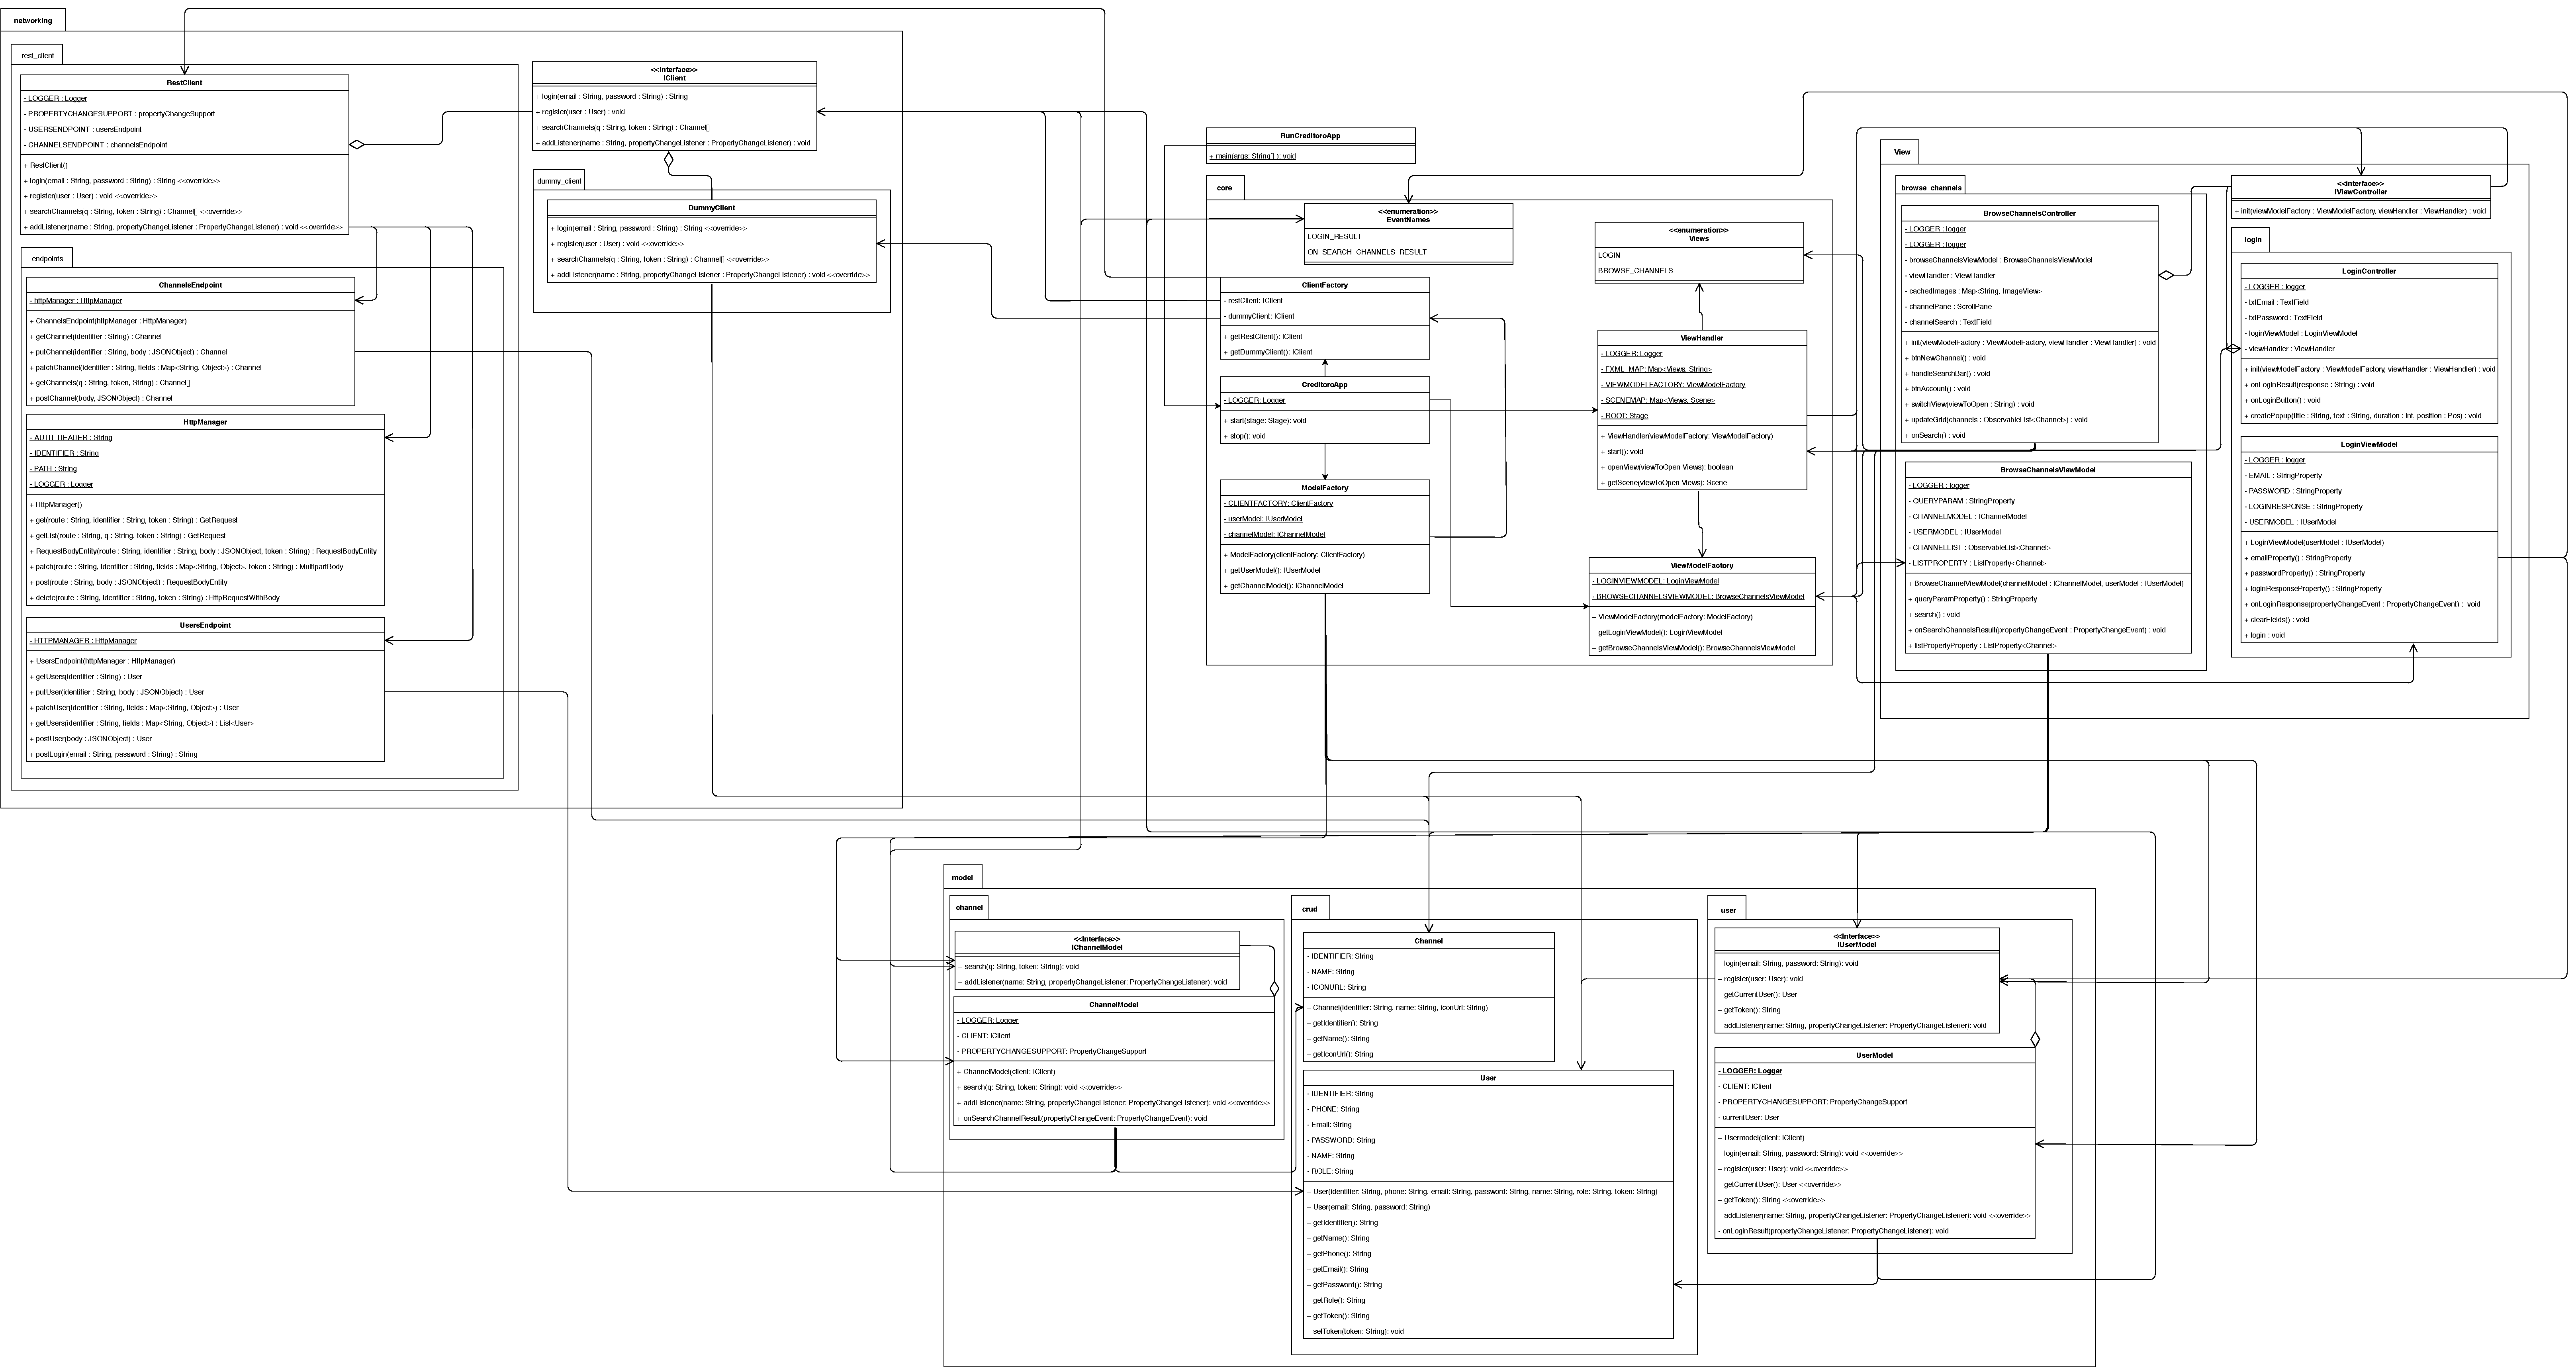
\includegraphics[fitpaper=true, scale=0.73]{figures/design/domaindiagram-Desktop Client_ UML med pile}\hspace*{\fill}
%\newpage
%\endgroup
\subsubsection{resultater}
        
        
\subsection{Softwarearkitektur}        
\subsubsection{Overvejelser}
\myworries{hvilke overvejelser havde vi i forhold til strukturen af hele systemet og hvordan kom vi frem til diagramet} \\
Gruppen startede med at kigge projekte caset igennem. \cite{TV2-case} \hyperlink{https://docs.google.com/document/d/1p6lQjWV76TX9uTLst2OAdmV07XfMRn5fObelzBpd2EI/edit}{Projekt case} var det første der blev omtalt. Der blev snakket meget om vi kunne nå at lave et Rest API.

\subsubsection{Beslutninger}
\subsubsection{resultater}

\begin{figure}[h]
    \centering
    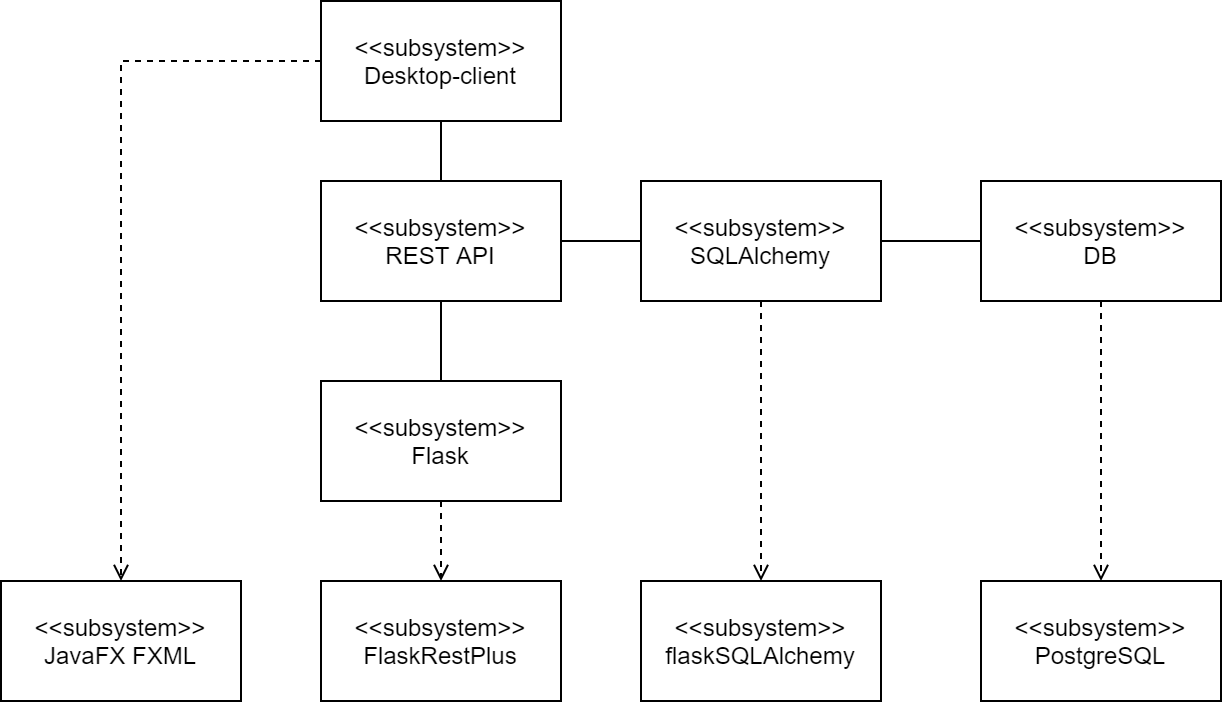
\includegraphics[width=\textwidth]{figures/design/domaindiagram-Software Architecture Diagram.png}
    \caption{Domaindiagram Software Architecture Diagram}
    \label{fig:domaindiagram-software-diagram}
\end{figure}{}
